\chapter{Architecture Dimensioning}
\label{chap:conv_gemm_equiv}

\section{Layer Equivalence}

Accelerator generality can be maintained by supporting general matrix
multiplication operations as well as convolution operations common in many
modern deep neural networks. Convolution operations can be converted into
general matrix multiplication through the use of lowering and lifting techniques
like Im2col discussed in \cite{cafe_con_troll}. To support matrix multiplication
within a convolution accelerator we can reporpose existing compute and memory
hardware on chip to perform both GEMM and convolutions operations or we can
establish a mathematical equivelence between GEMM operations and Conv by
reinterpret GEMM into a special case of convolution, namely convolutions with a
1x1 kernel size. This avoids the overhead of reporposing existing convolution
hardware to support GEMM. In \autoref{chap:conv_gemm_equiv:proof}, a proof for
the equivelence between GEMM and 1x1 Convolutions is given. Additionally, in
\autoref{chap:conv_gemm_equiv:application} the afformentioned proof will be used
in tandem with the approach in \cite{cafe_con_troll} to provide support for
arbitrary convolution operations. Finally in
\autoref{chap:conv_gemm_equiv:overhead} a discussion of the overheads associated
with the approach in \autoref{chap:conv_gemm_equiv:application} is given.

\clearpage

\subsection{Functional equivelence between GEMM and 1x1 Convolutions}
\label{chap:conv_gemm_equiv:proof}

We can establish functional equivelence between GEMM and 1x1 convolutions with
the following proof. An illustration of this proof is given in
\autoref{fig:gemmTo1x1Conv}.  
Given two matricies $A\in \mathbb{R}^{Z \times C}$ and $B \in \mathbb{R}^{C
\times F}$, let $R \in \mathbb{R}^{Z\times F} = A.B$. A different way to express
the matrix multiplication $A.B$ is \autoref{math:gemm_array_notation}.  

\begin{equation}
    \begin{aligned}
        R[z][f] = \displaystyle\sum\limits_{c=0}^{C-1}A[z][c]\times B[c][f] \\ \forall z\in[0, n^2-1]
    \end{aligned}
    \label{math:gemm_array_notation}
\end{equation}

Transposing $A$ and $B$ yields $\hat{A} \in \mathbb{R}^{C\times Z}$ and $\hat{B} \in
\mathbb{R}^{F\times C}$. Using the identity $(A.B)^T = B^T.A^T$ we can rewrite
\autoref{math:gemm_array_notation} as
\autoref{math:gemm_array_notation_transpose} where $\hat{R} \in
\mathbb{R}^{F\times Z}$

\begin{equation}
    \begin{aligned}
        \hat{R}[f][z] = \displaystyle\sum\limits_{c=0}^{C-1}\hat{B}[f][c]\times \hat{A}[c][z] \\ \forall z\in[0, Z-1]
    \end{aligned}
    \label{math:gemm_array_notation_transpose}
\end{equation}

We can reshape $\hat{A}$ and $\hat{B}$ using \autoref{math:a_b_reshape} into 3D
tensors by adding an additional dimention of size 1 for $\hat{A}$ and 2
additional dimentions of size 1 for $\hat{B}$.

\begin{equation}
    \begin{aligned}
        \hat{A} \xrightarrow[]{Reshape} &\hat{A}  \in \mathbb{R}^{C \times Z\times 1}   &\hat{B} & \xrightarrow[]{Reshape} \hat{B}  \in \mathbb{R}^{F \times C\times 1\times 1} \\
    \end{aligned}
    \label{math:a_b_reshape}
\end{equation}

Applying \autoref{math:a_b_reshape} to
\autoref{math:gemm_array_notation_transpose} yields
\autoref{math:gemm_as_conv_1} where $\hat{R} \in \mathbb{R}^{F \times Z\times 1}
$ remains the transposed output of $A.B$. 

\begin{equation}
    \begin{aligned}
        \hat{R}[f][z][0] = \displaystyle\sum\limits_{c=0}^{C-1}\hat{A}[c][z][0]*\hat{B}[f][c][0][0] \\ \forall z \in [0, Z-1] 
        \end{aligned}
    \label{math:gemm_as_conv_1}
\end{equation}

Adding kernel summations to \autoref{math:gemm_as_conv_1} yields
\autoref{math:gemm_as_conv_2} which is equivelent to a 1x1 convolution of stride
1. To recover $R$ from $\hat{R}$ we can reshape $\hat{R}$ by removing the
last dimention and then transpose it. 

\begin{equation}
    \begin{aligned}
        \hat{R}[f][z][0] = \displaystyle\sum\limits_{c=0}^{C-1}\displaystyle\sum\limits_{k_x=0}^{1} \displaystyle\sum\limits_{k_y=0}^{1}\hat{A}[c][y+ky][x+kx]*\hat{B}[f][c][k_y][k_x] \\ \forall y \in [0, Z-1] \land x = 0
    \end{aligned}
    \label{math:gemm_as_conv_2}
\end{equation}

\begin{figure}[]
    \centering
    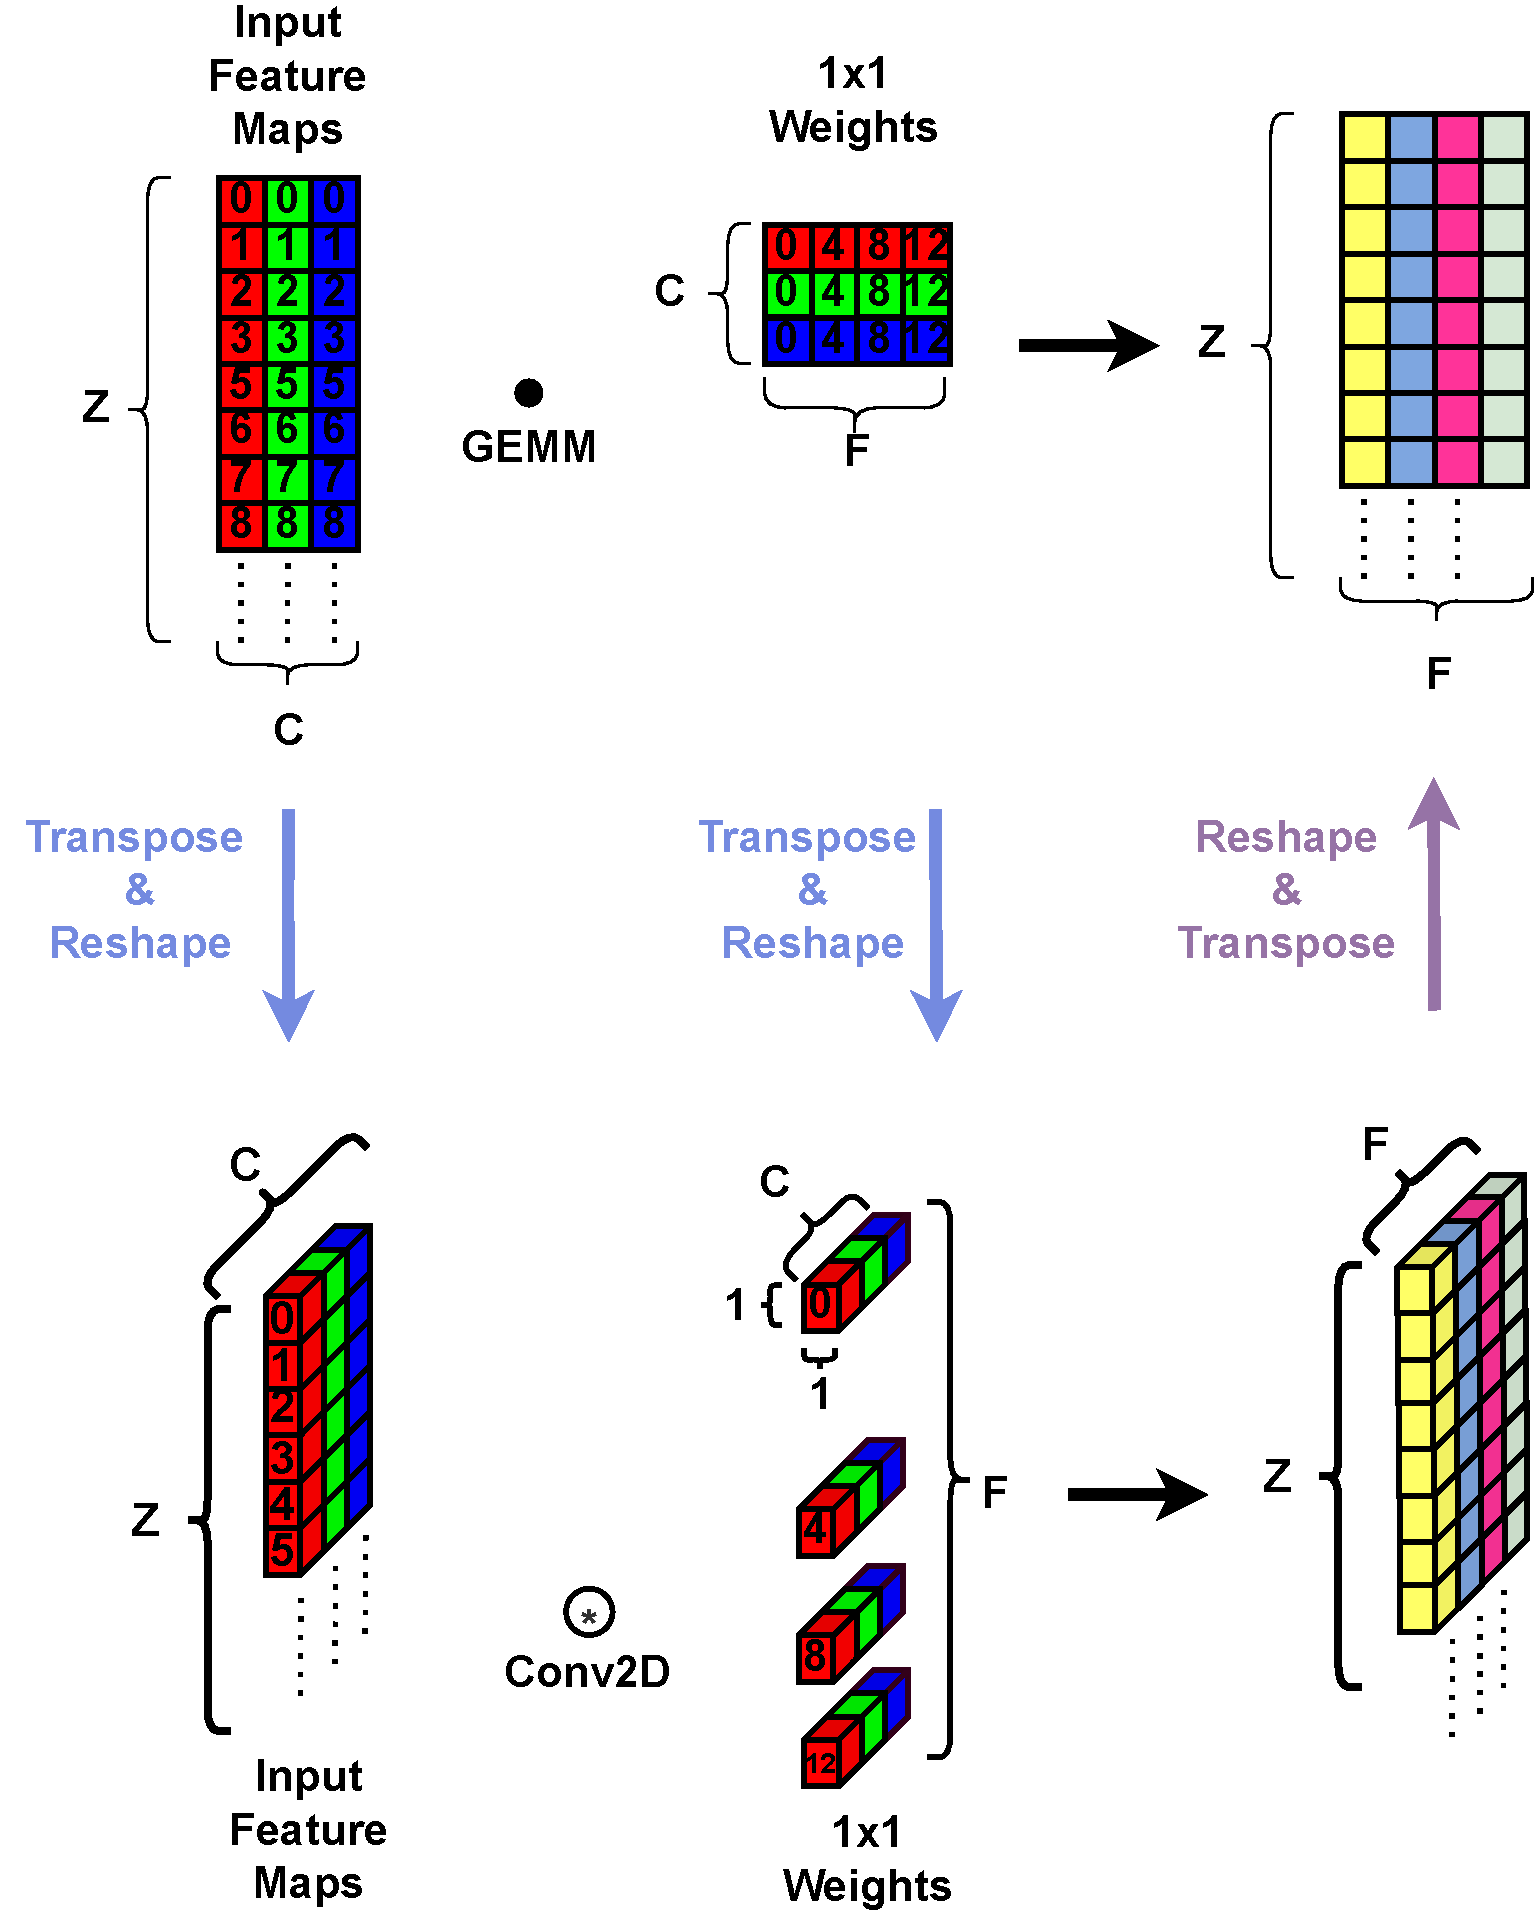
\includegraphics[scale=0.5]{fig/GemmTo1x1Conv.pdf}
    \caption{\ac{GEMM} and 1x1 Convolution Equivelence}
    \label{fig:gemmTo1x1Conv}
\end{figure}


\subsection{Supporting unsupported kernel sizes in a direct convolution accelerator}
\label{chap:conv_gemm_equiv:application}

We can support previously unsupported kernel sizes by combining the GEMM to 1x1
Conv conversion in \autoref{chap:conv_gemm_equiv:proof} with any tensor
lowering/lifting approach in \cite{cafe_con_troll}. Lowering converts a
convolution into a GEMM operation, and the approach in
\autoref{chap:conv_gemm_equiv:proof} reinterprets that operation as another 1x1
Convolution. This approach allows any convolution accelerator that can support
1x1 convolution operations to support any arbitrary convolution operation. A
visual illustration for this technique is presented in \autoref{fig:conv2gemm2conv}.
To demonstrate this approach we begin by lowering both IFmap using
\autoref{math:balanced_lowering_ifmap} and Weights using
\autoref{math:balanced_lowering_weight}. This results in two matricies IFmap and
Weights in \autoref{math:conv2gemm2conv:lowering}. Lowering should be performed
if the kernel size of the Weight tensor is unsupported $K' \notin
\{SupportedKernels\}$. 

\begin{equation}
    \begin{aligned}
        IFmap \in R^{C\times n\times n} & \xrightarrow[]{Balanced Lowering} \hat{IFmap} \in R^{nm\times K'C} \\
        Weight \in R^{F\times C\times K' \times K'} & \xrightarrow[]{Balanced Lowering} \hat{Weight} \in R^{K'C\times K'F} \\
    \end{aligned}
    \label{math:conv2gemm2conv:lowering}
\end{equation}

After lowering both tensors, we apply the transformations in
\autoref{math:conv2gemm2conv:transform} to reinterpret the anticipated GEMM
operation that occurs after lowering into a 1x1 convolution operation. The
transformations are composed of a transpose operation followed by a reshape
operation that appends additional dimentions of size 1 to both IFmap and
Weights. The transformations yields two new tensors $\hat{IFmap}$ and
$\hat{Weight}$.

\begin{equation}
    \begin{aligned}
        \hat{IFmap}^T \in R^{K'C \times nm} & \xrightarrow[]{Reshape} \hat{IFmap} \in R^{K'C \times nm \times 1} \\
        \hat{Weight}^T \in R^{K'F\times K'C} & \xrightarrow[]{Reshape} Weight \in R^{K'F\times K'C \times 1 \times 1} \\
        \end{aligned}
    \label{math:conv2gemm2conv:transform}
\end{equation}

After performing the transformations in \autoref{math:conv2gemm2conv:transform}
the output $\hat{OFmap_{prelift}}$ can be calculated after performing a 1x1
convolution in \autoref{math:conv2gemm2conv:conv} using the $\hat{IFmap}$ and
$\hat{Weight}$ tensors. 

\begin{equation}
    \begin{aligned}
        \hat{OFmap_{prelift}} \in R^{K'F\times nm \times 1} = \hat{IFmap}*\hat{Weight}
        \end{aligned}
    \label{math:conv2gemm2conv:conv}
\end{equation}

Finally we can lift $\hat{OFmap_{prelift}}$ by first reshaping it into a 2D
matrix by dropping the last dimension and then transposing it. After that, we
can apply balanced lifting in \autoref{math:balanced_lifting_ofmap} to get the
final OFmap in \autoref{math:conv2gemm2conv:lift}.

\begin{equation}
    \begin{aligned}
        \hat{OFmap_{prelift}} \in R^{K'F \times nm \times 1} \xrightarrow[]{Reshape} OFmap_{prelift} \in R^{K'F\times nm} \\
        OFmap_{prelift}^T \in R^{nm\times FK} \xrightarrow[]{Balanced Lifting} OFmap \in R^{F \times m \times m} \\
            \end{aligned}
    \label{math:conv2gemm2conv:lift}
\end{equation}

\begin{figure}[]
    \centering
    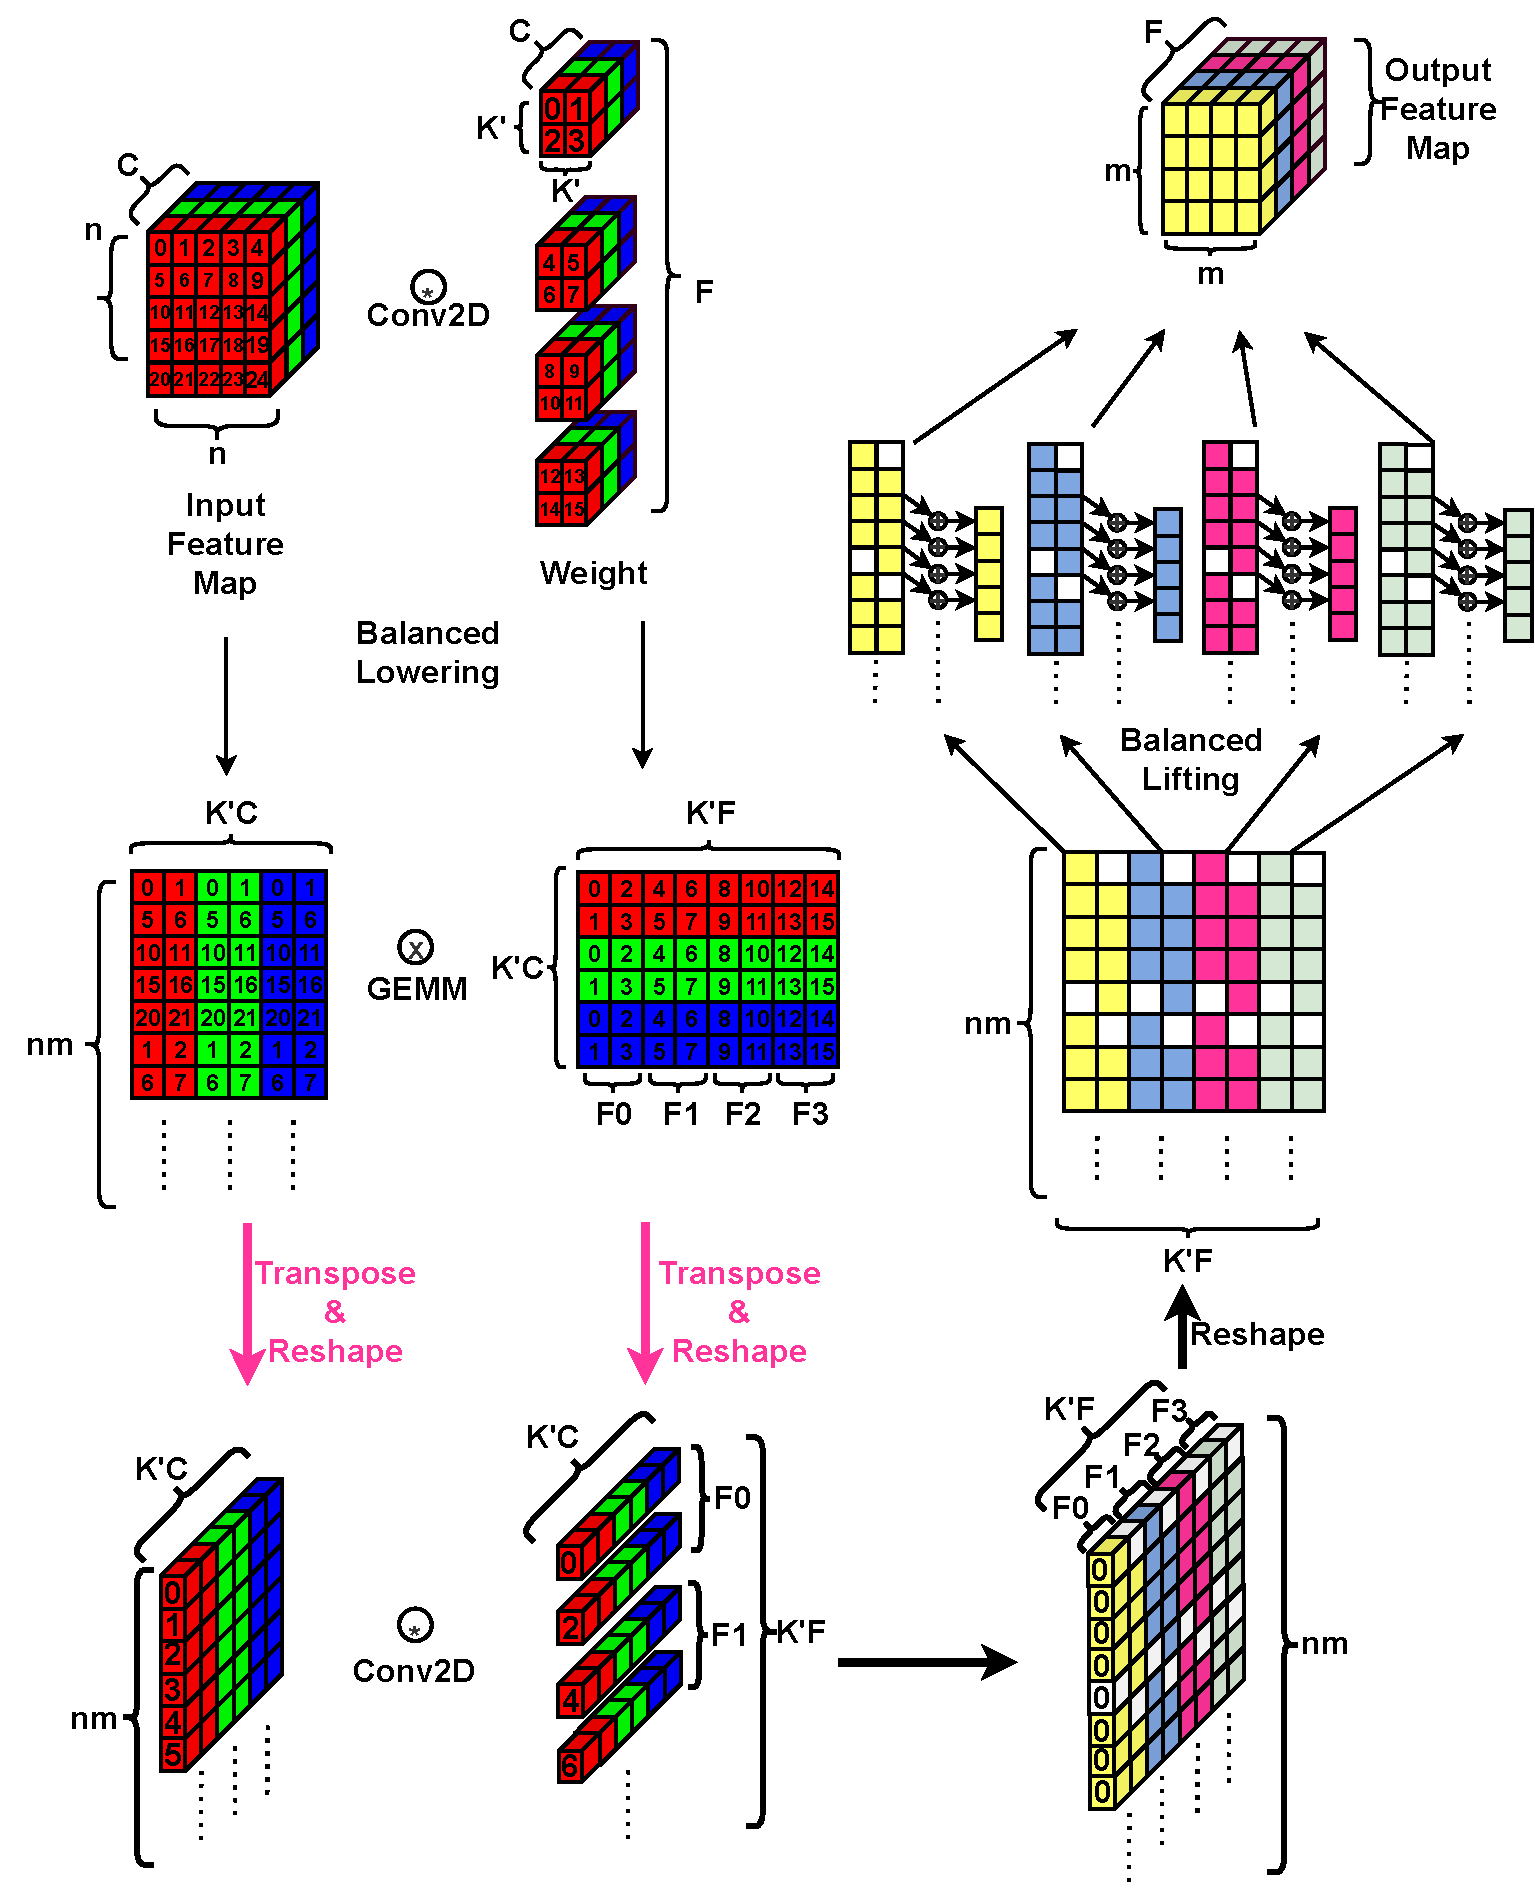
\includegraphics[scale=0.5]{fig/ConvToGemmToConv.pdf}
    \caption{Illustration of approach Conv2Gemm2Conv approach}
    \label{fig:conv2gemm2conv}
\end{figure}

\subsection{Overhead of extending support}
\label{chap:conv_gemm_equiv:overhead}

Lowering and lifting introduce additional overheads with regards to latency and
tensor sizing. The latency for performing balanced lowering and lifting is
$m^{2}K$ for a layer with a Weight tensor $\mathbb{R}^{F\times C\times K\times
K}$ and an OFmap tensor $\mathbb{R}^{F\times m\times m\times}$. While lowering
and lifting can be performed by a convolutions accelerator, in this thesis it is
assumed that a software processor on the same chip performs these operations.
Lowering also introduces duplicate data elements in the IFmap tensor thus
increasing it's overall size. In this thesis, it is assumed that on-chip memory
can account for this increase and that any additional DRAM accesses incurred
from lowering will be included in energy calculations when reporting energy
consumption of the accelerator.

To enable GEMM operations using the approach in
\autoref{chap:conv_gemm_equiv:proof} both input and output matricies are
transposed and reshaped. All reshape operations discussed in this chapter add a
dimention of size 1 to the data and they incur no data reorganization overhead.
Additionally, all transpose operations are assumed to be performed during
transfer to and from accelerator on-chip and thus incur no latency penalty. A
discussion of how transfers to and from on-chip memory can mask the latency of
transposing matricies is left as part of future work along with incorporating
lowering and lifting into the accelerator. 

% TODO: Mention savings as percentage of im2col
% https://www.desmos.com/calculator/p1qhtddjpa


\section{Exploring the dataflow design space with TEMPO}
\label{chap:dataflow_dse:exploring}

\begin{figure}[]
    \centering
    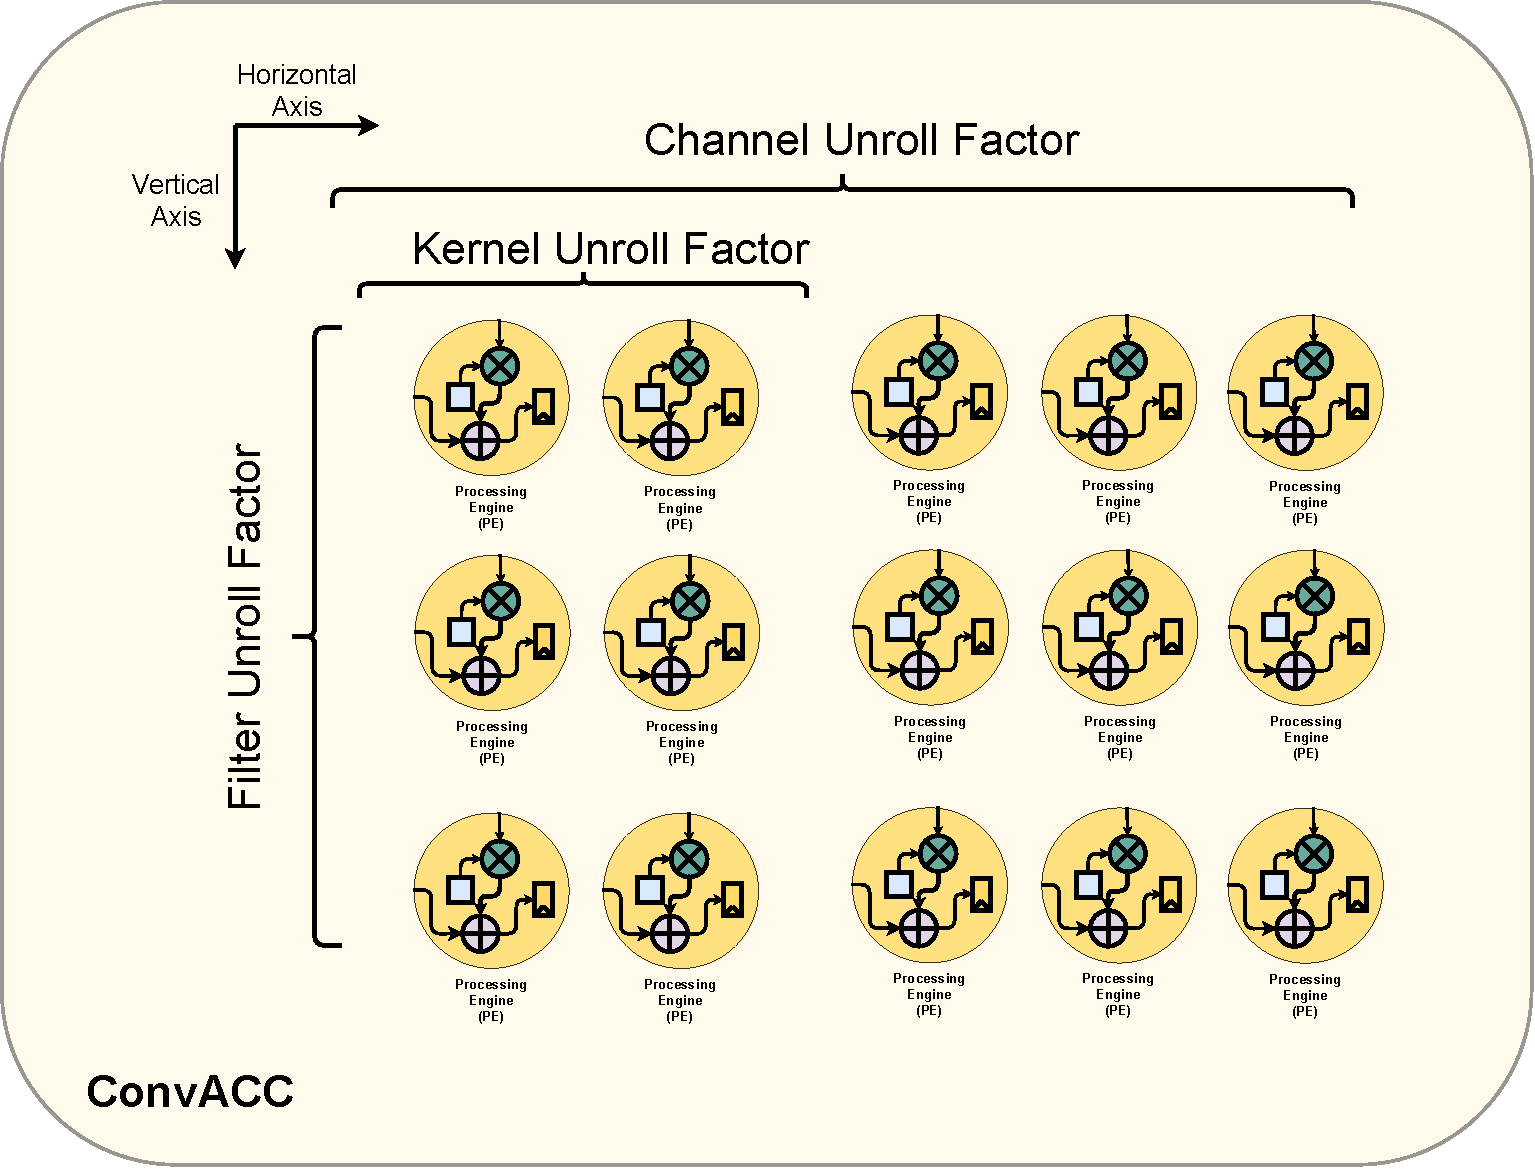
\includegraphics[scale=0.4]{fig/axis_mapping.pdf}
    \caption{\ac{GEMM} and 1x1 Convolution Equivelence}
    \label{fig:axis_mapping}
\end{figure}

From the previous section we have concluded that loops F, C, KY and KX are all
unroll targets, and KY and KX loops should be unrolled assuming that 1x1 and 3x3
kernels are supported directly. Additionally, the loop ordering of F and C loops
was discussed as well as it's implications with regards to on-chip memory
sizing. What remains of the dataflow design space is the unroll factors for F
and C loops as well as the accelerator spatial axis mapping for all unrolled
loops F, C, KY, KX. From this point these parameters will be referred to as
accelerator template paremeters from which a concrete accelerator instance can
be defined. These accelerator template parameters define the number of
processing engines allocated to process channels, filters, and kernels
concurrently in the concrete architectures. An illustration of this \ac{PE}
allocation is present in \autoref{fig:axis_mapping}. The space of possible
unroll factors is as large as the space of possible loop upperbounds for the
afformentioned unrolled loops. However, as discussed earlier, some combinations
of loop upperbounds are unlikely in real networks. Additionally, spatial axis
mapping affects the effective unroll factors when executing different
convolution layers than the ones assumed when unrolling said loops. This further
expands the design space of a concrete accelerator's template parameters. To
effectively explore the space of loop unroll factors and accelerator spatial
axis mapping we introduce \ac{TEMPO}, a dataflow exploration and analysis tool
used to optimize an accelerator's weight stationary dataflow based on a target
CNN library as well as an arbitrary objective function. A discussion of
\ac{TEMPO}'s algorithm model is presented in
\autoref{chap:dataflow_dse:exploring:algorithm} as well as it's analytical model
in in \autoref{chap:dataflow_dse:exploring:tempo_model}. Additionally, results
of running \ac{TEMPO} on CIGAR's library of CNNs are presented in
\autoref{chap:dataflow_dse:exploring:results}. 

\subsection{TEMPO Algorithm}
\label{chap:dataflow_dse:exploring:algorithm}

TEMPO's algorithm is presented in algorithm \ref{alg:tempo_algo}. TEMPO explores the
space of possible filter and channel unroll factors as well as kernel axis
mappings by exhaustively iterating through the space of possible values. TEMPO
expects the following inputs. 

\begin{itemize}
\item Processed $model^{stats}_{dict}$ from CIGAR
\item An objective function $obj\_fn$
\item Maximum $pe_{budget}$ 
\item Set of kernels supported directly  $kernels_{supported}$ 
\end{itemize}

Tempo then produces an optimal filter, channel unroll factors and kernel axis
mapping that maximizes the given objective function under the $pe_{budget}$
constraint specified. 

In algorithm \ref{alg:tempo_algo} TEMPO effectively runs an optimization program
that performs the optimization in \autoref{math:tempo_algo_tldr} where for some
arbitrary objective function $obj\_fn$ is evaluated using some template config and
the model library. The objective function is a function that evaluates an
architectures score based on any of metrics discussed in
\autoref{chap:dataflow_dse:exploring:tempo_model} and layers in the model
library $model^{stats}_{dict}$. Prior to the search being performed algorithm
\ref{alg:tempo_algo} converts all layer not supported directly in the model to
1x1 equivelent layers based on the method discussed in
\autoref{chap:conv_gemm_equiv}.

\begin{equation}
    \begin{aligned}
        \operatorname*{argmax}_{f_{unroll}, c_{unroll}, k_{axis}} obj\_fn(f_{unroll}, c_{unroll}, k_{axis}, ModelLibrary) \\
        \text{subject to} \\
        F_{unroll}. C_{unroll} <= Pe_{budget}
    \end{aligned}
    \label{math:tempo_algo_tldr}
\end{equation}

\begin{algorithm}[H] 
    \caption{\ac{TEMPO}}
    \label{alg:tempo_algo}
    \begin{algorithmic}[1]
    \Require{$model^{stats}_{dict}$, $obj\_fn$, $kernels_{supported}$, $pe_{budget}$} 
    \Ensure{$template^{opt}_{config}$}
    \Statex
    \Function{TEMPO\_run}{$model^{stats}_{dict}$, $obj\_fn$, $kernels_{supported}$, $pe_{budget}$}
        \State $max_{score} \gets -\inf$
        \State $template_{opt} \gets nil$
        \State $\hat{model^{stats}_{dict}} \gets convert\_all\_unsupported\_layers(model^{stats}_{dict}, kernels_{supported})$
        \For{$f_{unroll} \gets factors(pe_{budget})$}
            \For{$k_{axis} \gets \{Verticle, Horizontal\}$}
                \State $c_{unroll} \gets \lfloor \frac{pe_{budget}}{f_{unroll}} \rfloor$ 
                \State $template_{score} \gets obj\_fn(f_{unroll}, c_{unroll}, k_{axis}, \hat{model^{stats}_{dict}})$
                \If{$max_{score} < template_{score}$}
                    \State $max_{score} \gets template_{score}$
                    \State $template_{opt} \gets template_{config}$
                \EndIf
            \EndFor
        \EndFor
        \State \Return {$template^{opt}_{config}$}
    \EndFunction
    \end{algorithmic}
\end{algorithm}

\subsection{TEMPO analytical model}
\label{chap:dataflow_dse:exploring:tempo_model}

\subsubsection{Layer equivelence}
\label{chap:dataflow_dse:exploring:tempo_model:layer_equivelence}

In TEMPO's analytical model, an automatic layer conversion step is performed to
change the dimensionality of the IFmap and Weight tensors on the basis of
whether a layer's kernel size is supported directly or not. This conversion
follows the approach outlined in \autoref{chap:conv_gemm_equiv} which is used to
extend support to unsupported convolution layers. Wheather or not a convolution
layer's kernel size is supported directly has an effect on the assumed
dimensionalities of the IFmap and Weight tensors as well as the kernel loops
unroll factor K. Kernels are assumed to be symmetric so both kernel KY and KX
loops and share a single unroll factor $K_{unroll}$. If the convolution layer's
kernel size is supported directly no changes are assumed to have been made to
the dimensionality of the input. The kernel unroll factor is then equal to the
kernel size of the layer in accordance with the conclusions drawn from
\autoref{chap:dataflow_dse:pruning:applying_it:loop_unroll_factors}. However, if
a convolutions layer's kernel size is not supported directly, the layer's kernel
size is converted to 1x1 as seen in \autoref{math:K_unroll_factor} and lowering
is assumed to have been performed on IFmap and Weight tensors in accordance with
the approach discussed in \autoref{chap:conv_gemm_equiv}. For a convolution
layer with IFmap dimensionality $R^{C\times n\times n}$, Weight dimensionality
$R^{F\times C\times K\times K}$ and OFmap dimensionality $R^{F\times m\times m}$
the layer's new filter count $\hat{F}$, channel count $\hat{C}$, and IFmap
channel size $\hat{Z}$ values are reflected in \autoref{math:layer_equivelence}. 

\begin{align}
    \begin{gathered}
        K_{unroll} = \begin{cases} K & K \in \{SupportedKernels\}\\1 &K \notin \{SupportedKernels\}\end{cases}
            \end{gathered}
    \label{math:K_unroll_factor}
\end{align}

\begin{align}
    \begin{gathered}
        \hat{C} = \begin{cases} C &  K \in \{SupportedKernels\}\\ CK & K \notin \{SupportedKernels\}\end{cases} \\
        \hat{F} = \begin{cases} F &  K \in \{SupportedKernels\}\\ FK & K \notin \{SupportedKernels\}\end{cases} \\
        \hat{Z} = \begin{cases} m^2 &  K \in \{SupportedKernels\}\\ nm & K \notin \{SupportedKernels\}\end{cases}
            \end{gathered}
    \label{math:layer_equivelence}
\end{align}

\subsubsection{Axis mapping}
\label{chap:dataflow_dse:exploring:tempo_model:axis_mapping}

When determining axis mapping, F and C loops are assumed to be bound to an
accelerator's verticle and horizontal spatial axis. Utilizing both axis results
in better overall on-chip area utilization assuming conventional 2 dimensional
constraints for chip fabrication. Mapping all loops to the same axis can provide
the most flexibility with regards to the allocation of PEs as a resource to
process different filters, channels and kernels. However, this complicates on
chip connectivity and is not considered by TEMPO. KY and KX loops can then be
bound to either the horizontal or veticle axis of an accelerator based on the
variable $K_{axis}$.  Depending on which axis KY and KX loops are mapped, the
effective unroll factors for F and C loops ($F_{eff}$ and $C_{eff}$) are
changed. If the unrolled kernel loops share the same axis as the C loops, the
effective $C_{unroll}$ factor for the C loops is then $\lfloor
\frac{C_{unroll}}{K_{unroll}} \rfloor$ which means the effective C unroll factor
decreases depending on the size of the kernel unroll factor. This decrease in
effective unroll factor arises from the fact that, within the same axis as the C
loops, \ac{PE}s are allocated to process a single $K^2_{unroll}$ kernel. This
results in a decrease of \ac{PE}s available to process other channels
concurrently. The same logic applies to F loops if the Kernel loops are mapped
to the same axis verticle axis as they are. This idea is presented in
\autoref{math:effective_unroll_factors_c} and
\autoref{math:effective_unroll_factors_f}. In both equations $F_{unroll}$ and
$C_{unroll}$ are the unroll factors for F and C loops assuming $KY=KX=K=1$.


\begin{align}
    \begin{gathered}
        C_{eff} = \begin{cases} \lfloor \frac{C_{unroll}}{K^{2}_{unroll}} \rfloor & K_{axis} = horizontal\\ C_{unroll} & K_{axis} = Verticle\end{cases} \\
        \end{gathered}
    \label{math:effective_unroll_factors_c}
\end{align}
\begin{align}
    \begin{gathered}
        F_{eff} = \begin{cases} \lfloor \frac{F_{unroll}}{K^{2}_{unroll}} \rfloor & K_{axis} = Verticle\\ F_{unroll} & K_{axis} = Horizontal\end{cases} \\
        \end{gathered}
    \label{math:effective_unroll_factors_f}
\end{align}

\subsubsection{Metric: Utilization}
\label{chap:dataflow_dse:exploring:tempo_model:utilization}

\begin{figure}[]
    \centering
    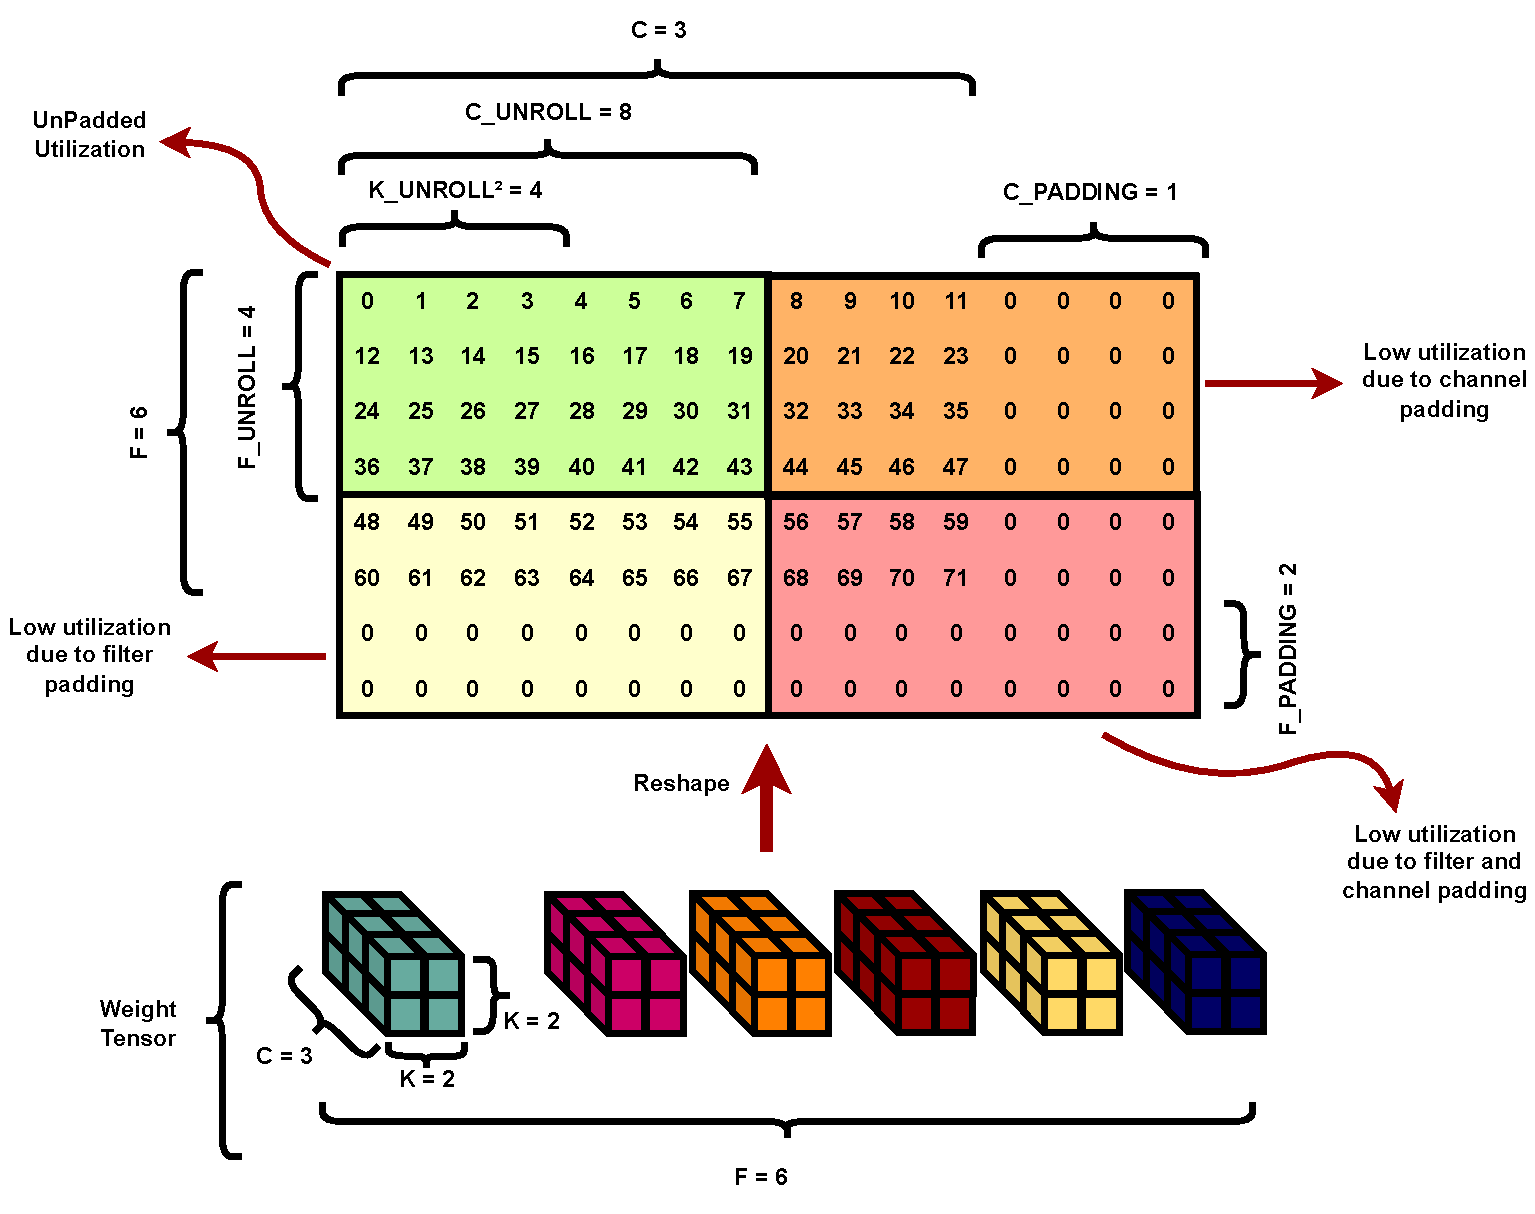
\includegraphics[scale=0.45]{fig/Lasso_ilus.pdf}
    \caption{\ac{GEMM} and 1x1 asd Equivelence}
    \label{fig:tempo_model}
\end{figure}

TEMPO models accelerator utilization based on how the template parameters (loop
unroll factors and loop axis mapping) tile and pad a convolution layer's
stationary weight tensor.  Kernel axis mapping is assumed to be inflexible
across accelerator spatial axis at runtime. An illustration of TEMPO's
utilization model in action is present in \autoref{fig:tempo_model}. In
\autoref{fig:tempo_model} a layer with a weight tensor of dimensionality
$R^{6\times 3\times 2\times 2}$ is tiled and padded based on the template
parameters $C_{unroll}=8$, $F_{unroll}=4$, $K_{unroll}=2$ and axis mapping
$K_{axis} = horizontal$. Based on these template parameters the effective filter
and channel unroll factors are $F_{eff} = 4$, $C_{eff}=2$. These unroll factors
create $\lceil \frac{\hat{C}}{C_{eff}} \rceil = 2$ horizontal tiles and $\lceil
\frac{\hat{F}}{F_{eff}} \rceil = 2$ verticle tiles assuming padding has been
applied. The weight tensor in \autoref{fig:tempo_model} is then reshaped into a
2D matrix of dimensionality $R^{8\times 16}$ with additional padding. The total
number of tiles is then reflected in \autoref{math:total_tiles}. 

\begin{align}
    \begin{gathered}
        Count_{Tiles} = \lceil \frac{\hat{F}}{F_{eff}} \rceil \lceil \frac{\hat{C}}{C_{eff}} \rceil
        \end{gathered}
    \label{math:total_tiles}
\end{align}

Utilization is calculated on a per-tile basis. There are two different types of
tiles, padded and unpadded, each with their own utilization calculation. Layer
utilization is then an average of the utilizations of each tile type weighted by
their frequency of occurence in the layer as reflect in
\autoref{math:layer_utilization}. For brevity each of the utilization equations
are multiplied by their frequency of occurence in the same equation. 

\begin{align}
    \begin{gathered}
        LayerUtilization = \frac{utilization^{UnPadded}_{Tiles} + utilization^{Padded}_{Tile(s)}}{Count_{Tiles}} \\
            \end{gathered}
    \label{math:layer_utilization}
\end{align}

The first tile type is the unpadded tile illustrated in
\autoref{fig:tempo_model} as the green tile. Utilization is calculated using
\autoref{math:tile_utilization_unpadded}. In this tile utilization is assumed to
be 1 and it's frequency of occurence depends on the number of unpadded tiles in
the layer $\lfloor \frac{\hat{F}}{F_{eff}} \rfloor \lfloor
\frac{\hat{C}}{C_{eff}}\rfloor$. 

\begin{align}
    \begin{gathered}
        utilization^{UnPadded}_{Tiles} = 1.\lfloor \frac{\hat{F}}{F_{eff}} \rfloor \lfloor \frac{\hat{C}}{C_{eff}}\rfloor \\
            \end{gathered}
    \label{math:tile_utilization_unpadded}
\end{align}

The second tile type is the padded tile of which there are three variations
depending on the reason for padding the tile. The utilization for all
padded tiles weighted by their frequencies of occurence is given in
\autoref{math:unpadded_tiles_weighted_average}. 

\begin{equation}
    \begin{aligned}
        utilization^{Padded}_{Tile(s)} & = utilization^{Padded}_{ChannelTiles} \\
                                       & + utilization^{Padded}_{FilterTiles} \\
                                       & + utilization^{Padded}_{ChannelAndFilterTiles} \\
    \end{aligned}
    \label{math:unpadded_tiles_weighted_average}
\end{equation}
  
If the allocation of PEs for channel loops exceeds avaliable channels to be
processed in the tile, then that tile will be padded. The padding in that tile results
in reduced PE utilization. An illustration of that padded tile variation is
present in \autoref{fig:tempo_model} as the orange tile.  The calculation for
the weighted utilization in that tile variation is given in equation
\autoref{math:tile_utilization_padded_channel}. To determine if a a padded channel
exists or not we can check if $\hat{C} \bmod C_{eff} > 0$ is true. If that
condition is true, padded channel tiles exist in the layer and their weighted
$utilization^{Padded}_{ChannelTiles}$ is then a function of how many PEs are
active in the tile $\frac{(\hat{C} \bmod C_{eff}) F_{eff}
K_{unroll}^2}{Count_{pe}}$ multipled by the frequency of occurence. $\lfloor
\frac{\hat{F}}{F_{eff}} \rfloor$. If $\hat{C} \bmod C_{eff} = 0$ then there are
no padded channel tiles so $utilization^{Padded}_{ChannelTiles} = 0$.

\begin{align}
    \begin{gathered}
        utilization^{Padded}_{ChannelTiles} = \begin{cases} \frac{(\hat{C} \bmod C_{eff}) F_{eff} K_{unroll}^2}{Count_{pe}}.\lfloor \frac{\hat{F}}{F_{eff}} \rfloor
         & \hat{C} \bmod C_{eff} > 0 \\ 0
         & \hat{C} \bmod C_{eff} = 0 \end{cases} \\
            \end{gathered}
    \label{math:tile_utilization_padded_channel}
\end{align}

If the allocation of PEs for filter loops exceeds avaliable filters to be
processed in the tile, then that tile will be padded. This another variation of
a padded tile and the weighted utilization for that tile variation is calculated
using \autoref{math:tile_utilization_padded_filter} and is illustrated in
\autoref{fig:tempo_model} as the yellow tile.

\begin{align}
    \begin{gathered}
        utilization^{Padded}_{FilterTiles} = \begin{cases} \frac{ C_{eff} (\hat{F} \bmod F_{eff}) K_{unroll}^2}{Count_{pe}}.\lfloor \frac{\hat{C}}{C_{eff}} \rfloor
            & \hat{F} \bmod F_{eff} > 0 \\ 0
            & \hat{F} \bmod F_{eff} = 0 \end{cases}
            \end{gathered}
    \label{math:tile_utilization_padded_filter}
\end{align}

Finally the last padded tile variation is the tile padded due to the excess
allocated of PEs for both filter and channel loops. This type of tile is
illustrated in \autoref{fig:tempo_model} as the red tile.  To determine if a tile like this
exists we can evaluate the condition $\hat{F} \bmod F_{eff} > 0 \land \hat{C}
\bmod C_{eff} > 0$ is true. If it there exists exactly one tile where
utilization is reduced due to excess allocation of PEs for filter and channel
loops. The equation to calculate weighted utilization in this padded tile
variation is given in \autoref{math:tile_utilization_padded_both}.

\begin{align}
    \begin{gathered}
         utilization^{Padded}_{Channel\&FilterTile} = \begin{cases} \frac{(\hat{C} \bmod C_{eff}) (\hat{F} \bmod F_{eff}) K_{unroll}^2}{Count_{pe}} & \hat{F} \bmod F_{eff} > 0 \land \hat{C} \bmod C_{eff} > 0 \\0  & else\end{cases}
            \end{gathered}
    \label{math:tile_utilization_padded_both}
\end{align}

\subsubsection{Metric: Latency}
\label{chap:dataflow_dse:exploring:tempo_model:latency}

Estimating latency follows the same tiling model discussed the previous
subsection. The latency of executing a layer based on the template paremeters
chosen is given in \autoref{math:latency}. Latency is a function of the number of
tiles present in the layer multiplied by the number of cycles spent processing a
single IFmap channel $\hat{Z}$ plus the additional latency incured due to
lowering lifting depending on the support for the layer's kernel size. Latency
for lowering and lifting is given in \autoref{math:latency_lowering_lifting}. If
the kernel is supported directly, no additional lowering and lifting penalties
are incurred, otherwise penalties are calculated based on the number of
operations necssary to lower the IFmap and Weight tensors plus the number of
operations to lift the OFmap. Lowering and lifting are assumed to be performed
by a software based co-processor. The latencies associated with lowering and
lifting can be eliminated if these operations are incoporated into the processor
however, that is left as part of future work. 

\begin{align}
    \begin{gathered}
        Latency = \hat{Z}.Count_{Tiles} + Latency_{Lowering} + Latency_{Lifting} \\
                \end{gathered}
    \label{math:latency}
\end{align}

\begin{align}
    \begin{gathered}
        Latency_{Lowering} = Latency_{Lifting} = \begin{cases} 0 &  K \in \{SupportedKernels\}\\ m^{2}K & K \notin \{SupportedKernels\}\end{cases} \\
                \end{gathered}
    \label{math:latency_lowering_lifting}
\end{align}

\subsubsection{Metric: Memory access counts}
\label{chap:dataflow_dse:exploring:tempo_model:access_counts}

Following the tiling model discussed earlier, memory access counts are
calculated based on how the template paremeters tile the layer's weight tensor.
Access counts for IFmaps are given in \autoref{math:memory_access_ifmap}, OFmap
access counts are giving in \autoref{math:memory_access_ofmap} and finally
weight access counts are given in \autoref{math:memory_access_weights}.

\begin{equation}
    \begin{aligned}
        IFmap^{AccessCount} = ((\hat{Z} K_{unroll}^2) (\lfloor\frac{\hat{C}}{C_{eff}} \rfloor C_{eff} + \hat{C}\bmod C_{eff}))\lceil\frac{\hat{F}}{F_{eff}}\rceil \\
    \end{aligned}
    \label{math:memory_access_ifmap}
\end{equation}
  
\begin{equation}
    \begin{aligned}
        OFmap^{AccessCount} = 2*\hat{Z} (\lfloor\frac{\hat{F}}{F_{eff}}\rfloor F_{eff}+\hat{F}\bmod F_{eff}) \lceil\frac{\hat{C}}{C_{eff}}\rceil \\
    \end{aligned}
    \label{math:memory_access_ofmap}
\end{equation}

\begin{equation}
    \begin{aligned}
        Weight^{AccessCount} & = \hat{Z}((C_{unroll}F_{unroll})(\lfloor\frac{\hat{C}}{C_{eff}} \rfloor \lfloor\frac{\hat{F}}{F_{Feff}}\rfloor) \\
            & +(C_{unroll}F_{eff})(\lfloor\frac{\hat{C}}{C_{eff}} \rfloor \hat{F}\bmod F_{eff}) \\
            & +(C_{eff}F_{unroll})(\lfloor\frac{\hat{F}}{F_{eff}} \rfloor \hat{C}\bmod C_{eff}) \\
            & + (C_{eff}F_{eff})(\hat{F}\bmod F_{eff}\space* \hat{C}\bmod C_{eff}))
        \end{aligned}
    \label{math:memory_access_weights}
\end{equation}

\subsection{TEMPO results}
\label{chap:dataflow_dse:exploring:results}

\subsubsection{Assumed objective function}
\label{chap:dataflow_dse:exploring:results:obj_fn}

Since TEMPO expects an objective function to maximize based on any or a
combination of all the discussed metrics in
\autoref{chap:dataflow_dse:exploring:tempo_model}
\autoref{math:tempo_results_obj_fn} defines an objective function based solely
on the average layer utilization metric over the entire set of convolution
layers in CIGAR's model library. Layer utilization is evaluated based on the
discussion in \autoref{chap:dataflow_dse:exploring:tempo_model:utilization}. 

\begin{equation}
        obj\_fn \gets average (\{LayerUtilization(layers)\space|\space \forall layers \in m, \forall m \in \{ModelLibrary\}\})
    \label{math:tempo_results_obj_fn}
\end{equation}

\begin{figure}[]
    \centering
    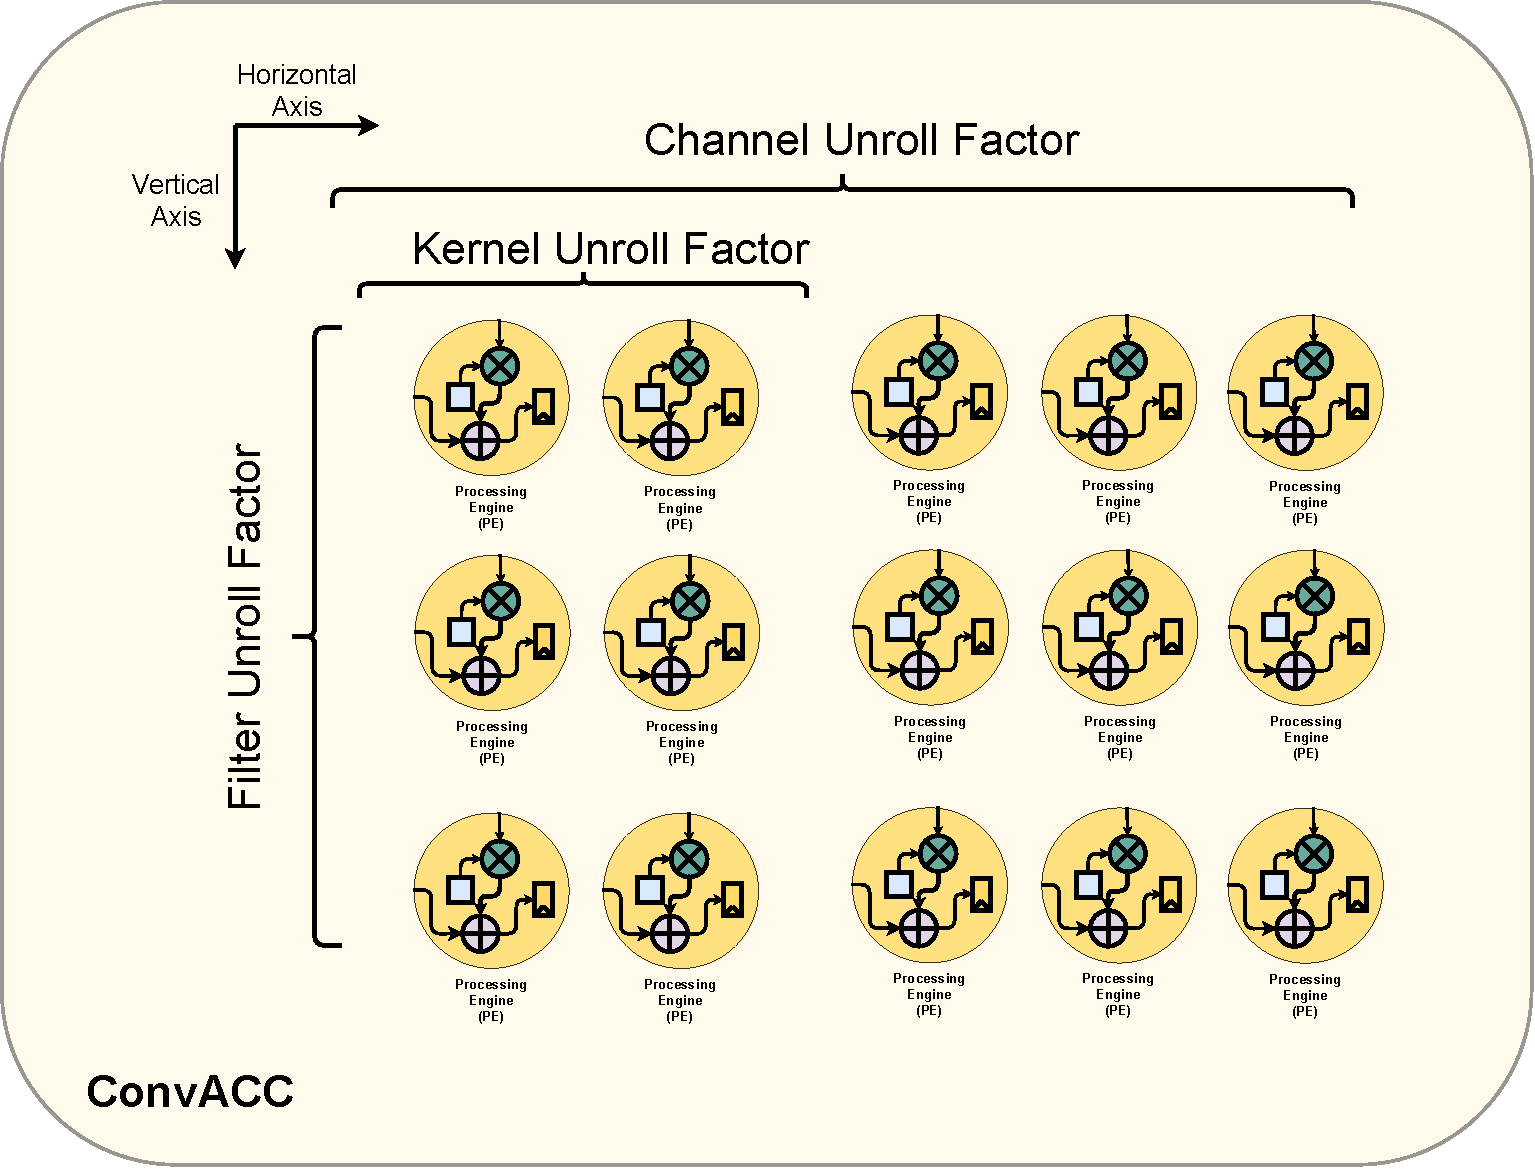
\includegraphics[scale=0.4]{fig/axis_mapping.pdf}
    \caption{\ac{GEMM} and 1x1 Convolution Equivelence}
    \label{fig:axis_mapping}
\end{figure}



% \State $arch_{config} \gets (f_{unroll}, c_{unroll}, k_{axis})$
% \For{$(model,\space layers) \in model^{stats}_{dict}$}
%     \For{$layer \in layers$}
%     \If{$layer.kernel\_size \notin kernels_{supported}$}
%         \State $\hat{layer} \gets supported\_layer\_equivelent(layer)$
%     \Else
%         \State $\hat{layer} \gets layer$
%     \EndIf
%     \State $layer_{metrics}.push (metrics\_fn(\hat{layer}, arch_{config}))$
%     \EndFor
% \EndFor 